\documentclass[10pt,twocolumn,letterpaper]{article}

\usepackage{statcourse}
\usepackage{times}
\usepackage{epsfig}
\usepackage{graphicx}
\usepackage{amsmath}
\usepackage{amssymb}
\usepackage{enumitem}
\graphicspath{ {./figures/} }

% Include otherhttps://www.overleaf.com/project/62015975f833a4b3efbe44ef packages here, before hyperref.

% If you comment hyperref and then uncomment it, you should delete
% egpaper.aux before re-running latex.  (Or just hit 'q' on the first latex
% run, let it finish, and you should be clear).
\usepackage[breaklinks=true,bookmarks=false]{hyperref}


\statcoursefinalcopy


\setcounter{page}{1}
\begin{document}


%%%%%%%%%%%%%%%%%%%%%%%%%%%%%%%%%%%%%%%%%%%%%%%%%%%%%%%%%%%%%%%
% DO NOT EDIT ANYTHING ABOVE THIS LINE
% EXCEPT IF YOU LIKE TO USE ADDITIONAL PACKAGES
%%%%%%%%%%%%%%%%%%%%%%%%%%%%%%%%%%%%%%%%%%%%%%%%%%%%%%%%%%%%%%%



%%%%%%%%% TITLE
\title{\ Poverty Estimation Using Satellite Images and Geospatial Data}

\author{Christine Cepelak\\
{\tt\small 216776@mds.hertie-school.org}
\and
Janine De Vera\\
{\tt\small janinepdevera@gmail.com}
\and
Johannes Halkenhäußer\\
{\tt\small halkenjo@gmail.com}
}

\maketitle
%\thispagestyle{empty}


% MAIN ARTICLE GOES BELOW
%%%%%%%%%%%%%%%%%%%%%%%%%%%%%%%%%%%%%%%%%%%%%%%%%%%%%%%%%%%%%%%

\newpage
\section{Introduction}
\subsection{Background}

Poverty is a multifaceted problem manifested by broad conditions such as malnutrition, homelessness, lack of access to clean water, and low educational achievement. It continues to be one the world’s most pressing issues and it has only been exacerbated by the economic effects of the COVID-19 pandemic. The United Nations’ Sustainable Development Agenda for 2015-2030 identifies poverty eradication as one of its top priorities – evidence that governments across the globe are committed to alleviating poverty. 

It follows that poverty statistics are among the most important and most widely used data in the economic and policy research sphere. Practical and ground-level applications of poverty data include identification of vulnerable populations for rolling out interventions by humanitarian and development organizations. However, measuring and monitoring poverty is both conceptually and operationally challenging. Poverty measurement is commonly the responsibility of national statistics offices, but the capacity to produce accurate and frequent information varies widely depending on the country. Ironically, the most vulnerable economies in need of extensive and up-to-date poverty data are also those who lack the capacity to compile them. Countries in extreme poverty or in conflict often lack relevant survey data for several years. 

This project\footnote{GitHub respository: \url{https://github.com/ccepelak/ML-SS22}} aims to contribute to the research body on bridging poverty statistics measurement gaps, through the application of machine learning techniques in satellite images and open source spatial data. The proposed machine learning models will incorporate intuitive geospatial variables to facilitate insightful interpretations and comparisons of different factors associated with poverty. 


\subsection{Methodology Overview}

To measure actual on-the-ground situations, data from official Demographic and Health Surveys (DHS)\footnote{USAID DHS database: \url{https://www.dhsprogram.com/Countries}} or population censuses will be collected. As in related studies \cite{chen2011using, ledesma2020interpretable, zhao2019estimation, zhongming2020mapping}, a wealth index or poverty index will be constructed as the variable of interest and primary measure of poverty and economic wellbeing. This will serve as the ground-level truth that will be used in conjunction with geospatial covariates such as nighttime luminosity, population mobility, accessibility, connectivity, and consumer preferences. Information will be collected and processed based on pre-defined geographic clusters or grids within multiple countries of interest. \\

As a starting point for research, seven countries from the most poverty-stricken regions in the world have been selected:

\begin{itemize}[noitemsep]
    \item Guatemala (South America)
    \item Haiti (Carribean)
    \item Kenya (Africa)
    \item Mongolia (Central Asia)
    \item Nepal (South Asia)
    \item Pakistan (Middle East)
    \item Timor-Leste (Southeast Asia)
\end{itemize}

The goal is to find complete and representative data for each country, so the focus of the study may shift to neighboring economies as the project progresses. \\

Three models will be estimated using data from the chosen countries: 
\begin{enumerate}
    \item \emph{Baseline model}: A simple linear regression examines the effect of identified explanatory variables on the wealth index. \cite{ledesma2020interpretable, zhao2019estimation} A slightly more complex variation is a spatial regression that accounts for effects of geographical characteristics of observations. 
    \item \emph{Random forest}: A random forest regression estimates multiple regression trees using different combinations of variables and averages over several predictions. The primary objective of such an approach is improving model explainability and robustness. \cite{ledesma2020interpretable, zhao2019estimation}.
    \item \emph{Deep learning algorithm}: A Convolutional Neural Network (CNN) is commonly used for machine vision algorithms. Unlike regular neural networks CNNs use a convolutional and a pooling layer to extract information from a subspace of the image thus preserving some of the underlying structure of the image. \cite{zhongming2020mapping}

\end{enumerate}
\begin{figure}[h]
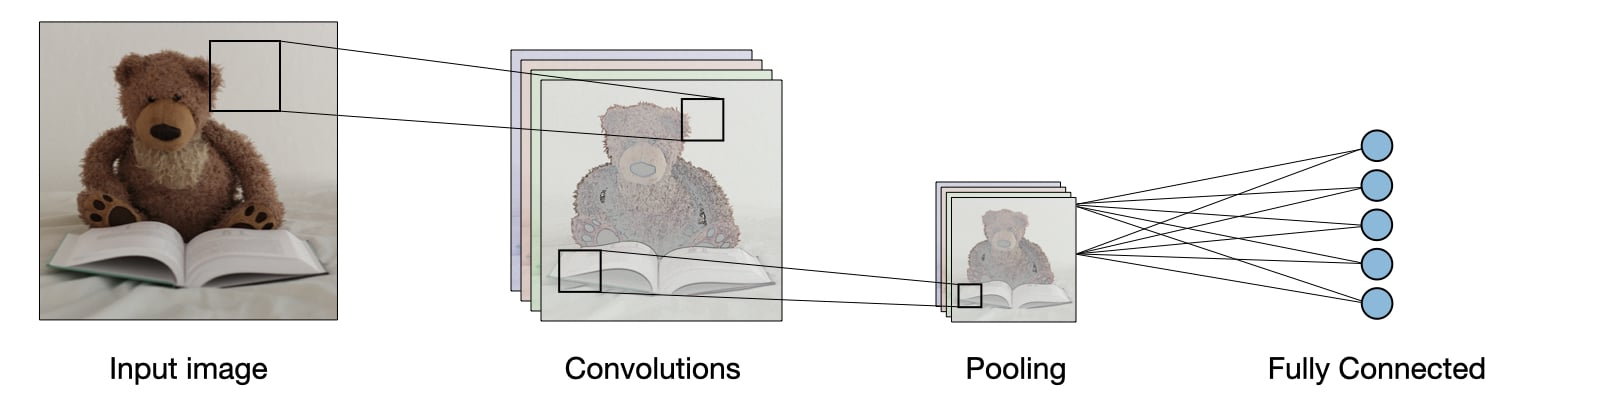
\includegraphics[scale=.16]{figures/architecture-cnn-en.jpeg}
\caption{The essential architecture of a convolutional neural network \cite{amidi_amidi_2019}.}
\label{fig:architecture-cnn-en}
\end{figure}

\section{Motivation}

As the world wrestles with the impacts of AI advancements and hyper connectivity on social media platforms, a basic foundation of governance is missing in many countries: accurate census data. As stated in the Background, the critical nature of addressing poverty needs no explanation; however, the urgent need to apply modern technological advances to basic social-political administration receives notably less attention. 

We hope these models can be applied to some of the most impoverished countries in the world. For example, Somalia and Afghanistan are in the small minority of countries which have not had a national census since 1990. Neighboring countries such as Pakistan and Kenya, however, have more substantial data available, which can be used to evaluate predictions. 

Without this type of census and poverty data, not only do countries lack the means to meaningfully support their own communities, but the international community cannot lend aid. 


\section{Evaluation}

Our motivation informs the goal outcome: a model with strong out of sample prediction and high external validity. An ideal model could hence be used to give an indication of where poverty is prevalent in countries that have outdated or poor quality census and survey data.

Success will mean to train a model that is in the realm of explanatory power as \cite{chen2011using, ledesma2020interpretable, zhao2019estimation} which achieve a $R^2$ of 0.66 and 0.70 respectively. The literature repeatedly refers to the $R^2$ as the evaluation metric, which we will hence adapt to evaluate our models likewise. The $R^2$ measures the variance in the dependent variable that can be explained by the independent variables. We will also use our model and predict poverty scores in a country not included in the training data and again report the $R^2$.

% Hey guys should we include the formula for R^2 here or is that too basic? 

\section{Resources}

There is a wealth of geospatial information that could potentially lend the proposed models more predictive power. Examples of geospatial variables and their data sources are summarized in Table \ref{table:1}. The list is preliminary and not exhaustive. \\

\begin{table}[h]
\begin{tabular}{p{0.7in}p{1.5in}p{0.8in}}
\hline
  \multicolumn{1}{c}{\textbf{Variable}} &
  \multicolumn{1}{c}{\textbf{Measurement}} &
  \multicolumn{1}{c}{\textbf{Sources}} \\ \hline
  Economic activity &
  Nighttime lights satellite images from remote sensing data &
  Google Earth Engine, QuickBird Imageries \\ \hline
  Population mobility &
  Population movement across different categories of places (e.g. workplace, residential, groceries and pharmacies, transit stations) &
  Google Mobility Report \\ \hline
  Accessibility &
  Distance from cluster centers to primary and secondary roads; counts of points of interests such as banks, schools, hospitals &
  OpenStreetMap \\ \hline
  Connectivity &
  Internet performance, stability, and speed &
  Ookla Open Datasets \\ \hline
  Consumer characteristics &
  Consumer goods preferences; number of Facebook users with breakdown per access segment (i.e. 4G, 3G, 2G, WiFi) &
  Facebook API \\ \hline
\end{tabular}
\caption{Geospatial variables and data sources.}
\label{table:1}
\end{table}

We will rely heavily on common machine learning libraries such as pandas and scikit-learn (data cleaning/wrangling, preprocessing, feature engineering, linear model, random forest) and keras (CNN). 

Granular satellite image data is quite large and hence we will preferably use the Google Data storage provided to us. Computationally, the final models should be trained using Hertie's GPUs. Setting up the pipeline can be done in Google Colab or on our devices with a subset of data. 

\section{Contributions}
We expect to work in close collaboration on realising our project. To that end we have set up a standing weekly call and will be splitting our workload according to our strengths. All three of us will work on procuring and harmonizing our data. To ensure that our models stay comparable, the pre-processing will also be worked on collaboratively while Janine and Christine will work on creating a clean data set, Johannes will work on the visualization of the data as well as relaying potential feature engineering or data anomalies back to the group. 
The models will be split by previous experience. Christine and Janine will develop the linear regression and the Random Forest model. Johannes has previously worked on NN and will focus on developing the convolutional neural network (CNN). 
The write-up/presentation will again be worked on together, yet each member of the group will be writing about the model they developed so no knowledge is lost between coding and write up. 

To ensure timely completion of the project, all members will follow the proposed timeline presented in Table \ref{table:2}. 

\begin{table}[h]
\begin{tabular}{cp{2.2in}}
\hline
\textbf{Date} & \multicolumn{1}{c}{\textbf{Deliverables}}                                              \\ \hline 
\multicolumn{2}{l}{\textit{\textbf{Preparatory work}}}                                                 \\ \hline 
wk 1 Mar      & Proposal submission; data gathering; finalization of countries to be included in study \\ \hline
wk 2 Mar      & Data gathering and cleaning                                                            \\ \hline
\multicolumn{2}{l}{\textit{\textbf{Exploratory analysis}}}                                             \\ \hline 
wk 3 Mar$^*$    & Exploratory data analysis; write up of initial findings                               \\ \hline
wk 4 Mar      & Finalization of mid-term report; Model 1 (Linear Regression)                            \\ \hline
\multicolumn{2}{l}{\textit{\textbf{Modeling}}}                                                         \\ \hline 
wk 1 Apr      & Model 2 (Random Forest), Model 3 (CNN) \\ \hline
wk 2 Apr$^*$ & Model 2 (Random   Forest), Model 3 (CNN) \\ \hline
\multicolumn{2}{l}{\textit{\textbf{Report and documentation}}}                                         \\ \hline
wk 3 Apr      & Finalization of analysis; documentation on Github; write up of final report            \\ \hline
wk 4 Apr      & Submission of final report; preparation for final presentation                         \\ \hline
wk 1 May      & Presentation                                                                           \\ \hline
\end{tabular}
\footnotesize{ $^*$ * Weeks when consultation meetings will be scheduled}
\caption{Proposed timeline of deliverables.}
\label{table:2}
\end{table}

\newpage
{\small
\bibliographystyle{ieee}
\bibliography{bibliography.bib}
}

\end{document}
